\chapter{国産民間ロケットの挑戦}

\section{はじめに}
MOMO,という名前のロケットがある.
「ホリエモンロケット」というと,聞いたことがあるかもしれない.
つい最近,今年の7月30日に初号機が打ち上げられたばかりのこのロケットは,北海道のベンチャー企業,インターステラ・テクノロジズが開発したロケットだ.
残念ながら初号機は宇宙空間に到達することは叶わなかったが,それでも離床には成功し,データの採取もできた.
そして,これは国内の民間企業では初の快挙である.
ここでは,このMOMOというロケットを開発したインターステラ・テクノロジズの歴史について少し調べたので書いてみようと思う.

\begin{figure}[htbp]
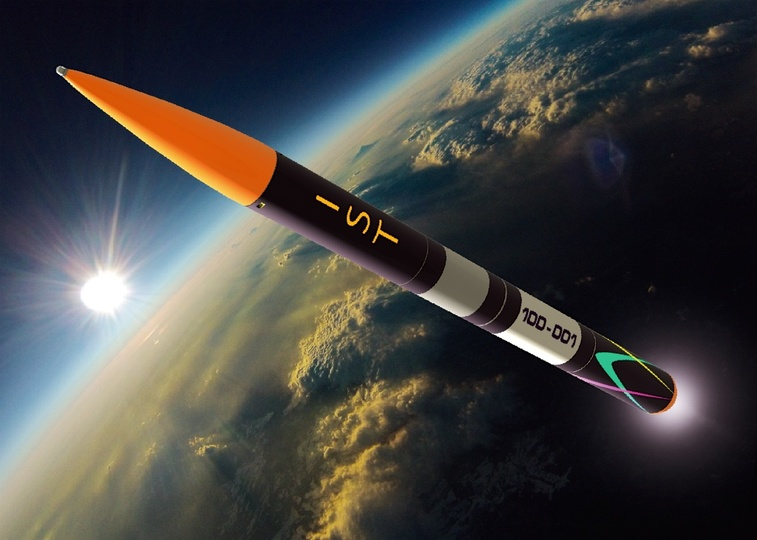
\includegraphics[width=5cm]{img/momo-rocket-image}
\caption{MOMOロケットのイメージ図}
\end{figure}

\section{はじまりは風呂場から}
1997年,H-Ⅱロケットを使用して,日本独自の有人宇宙船を打ち上げることはできないか,という検討会が,全国の宇宙好きの集まりで行われた.
その後,H-Ⅱではなく,既成のエンジンを使用した新型ロケットを作り,それを使って同様のことをやる計画が立ち上がった.宇宙に強い関心を持つ堀江貴文氏に出資をもちかけ,ロシアのロケットエンジンの購入を試みるも,全くアドバンテージがない不利な交渉となり,あまりの高額さから購入を断念する.


2005年,自分たちでロケットエンジンを作り,民間独自の低価格な小型ロケットを作ってしまおうという話になり,「なつのロケット団」
\footnote{「なつのロケット」はメンバーの一人である「あさり よしとお」氏の漫画のタイトル.}
を結成.
メンバーの住むアパートの風呂場で,最初期のロケットエンジンの試験を開始する.
\footnote{これが,「始まりは風呂場から」と言われる所以である.}

\section{繰り返す燃焼試験}
2006年,堀江氏当時社長を務めていたSNS株式会社の一事業としてロケットエンジンの開発に着手.2008年には30kgf級の最初のロケットエンジンの燃焼試験に成功,翌2009年に開発拠点を北海道に移し,90kgf級のエンジンの開発を開始.さらに2010年には100kgf級エンジンの開発に成功.
2011年には,最初のデモンストレーション打ち上げ機である「はるいちばん」他3機のロケットの打上試験に成功した.


2013年には,北海道大樹町にインターステラテクノロジズ株式会社を設立し,現在の体制となった.
インターステラテクノロジズ社は,大樹町にエンジン燃焼施設を整備し,本格的にエンジンの開発を進めた.
そして,純民間商業ロケット「ポッキー」,姿勢制御飛行実験機「LEAP」の打ち上げに成功.
さらに,高度100kmに到達する観測ロケット「MOMO」の開発を開始した.

\begin{figure}[htbp]
\centering
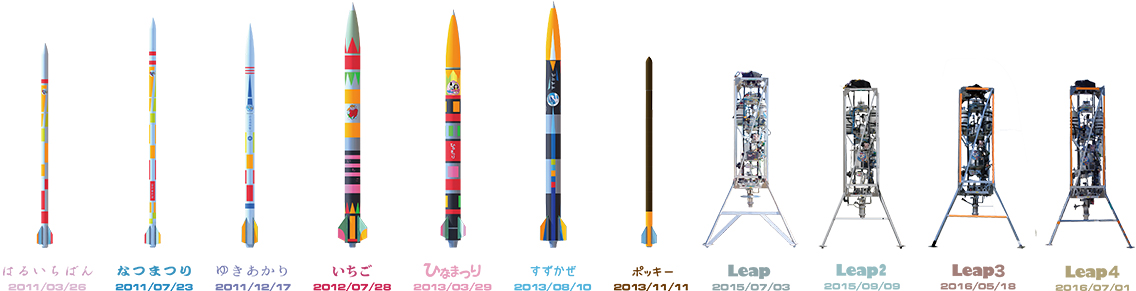
\includegraphics[width=10cm]{img/istellartech-rockets.jpg}
\caption{インターステラテクノロジズ社が開発したロケット}
\end{figure}

\section{インターステラのエンジン}
インターステラのロケットエンジンは,エタノールと液体窒素を燃料とした液体燃料方式だ.
これらの燃料は調達が容易であるため,頻繁な燃焼試験や,商用化した時の打ち上げコスト低下に大きく役立っている.


エンジンの構造は比較的単純で,燃料のタンクとは別に加圧用のヘリウムタンクを搭載して,ヘリウムガスの圧力で燃料を押し出し,インジェクターから混合・噴射,その後燃焼室で燃焼させて高圧の燃焼ガスを発生させ,グラファイト製のスロートで加速して噴き出す,というものだ.
\begin{figure}[htbp]
\centering
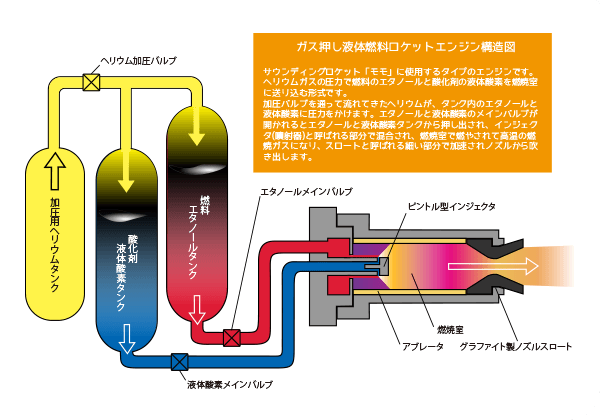
\includegraphics[width=7cm]{img/momo-engine.png}
\caption{ロケットエンジンの仕組み}
\end{figure}

\section{サウンディングロケット MOMO}
このように,独自のロケットエンジンの開発を主軸として民間でロケットを作り,打ち上げてきたインターステラ社だが,同社がつい最近,7月30日に打ち上げ実験を行ったのが,サウンディングロケット,「MOMO」だ.


サウンディングロケットというのは,弾道飛行を行う観測ロケットのことで,MOMOでは20kgまでの実験・観測機器をペイロードとして搭載し,高度100kmを目指す.
ペイロードはパラシュートで回収出来るため,気球などでは到達が難しい高高度の観測や,微小重力状態での実験を行うことができる.
\footnote{MOMOでは260秒間の微小重力状態を作り出すことが可能.}

\begin{figure}[htbp]
\centering
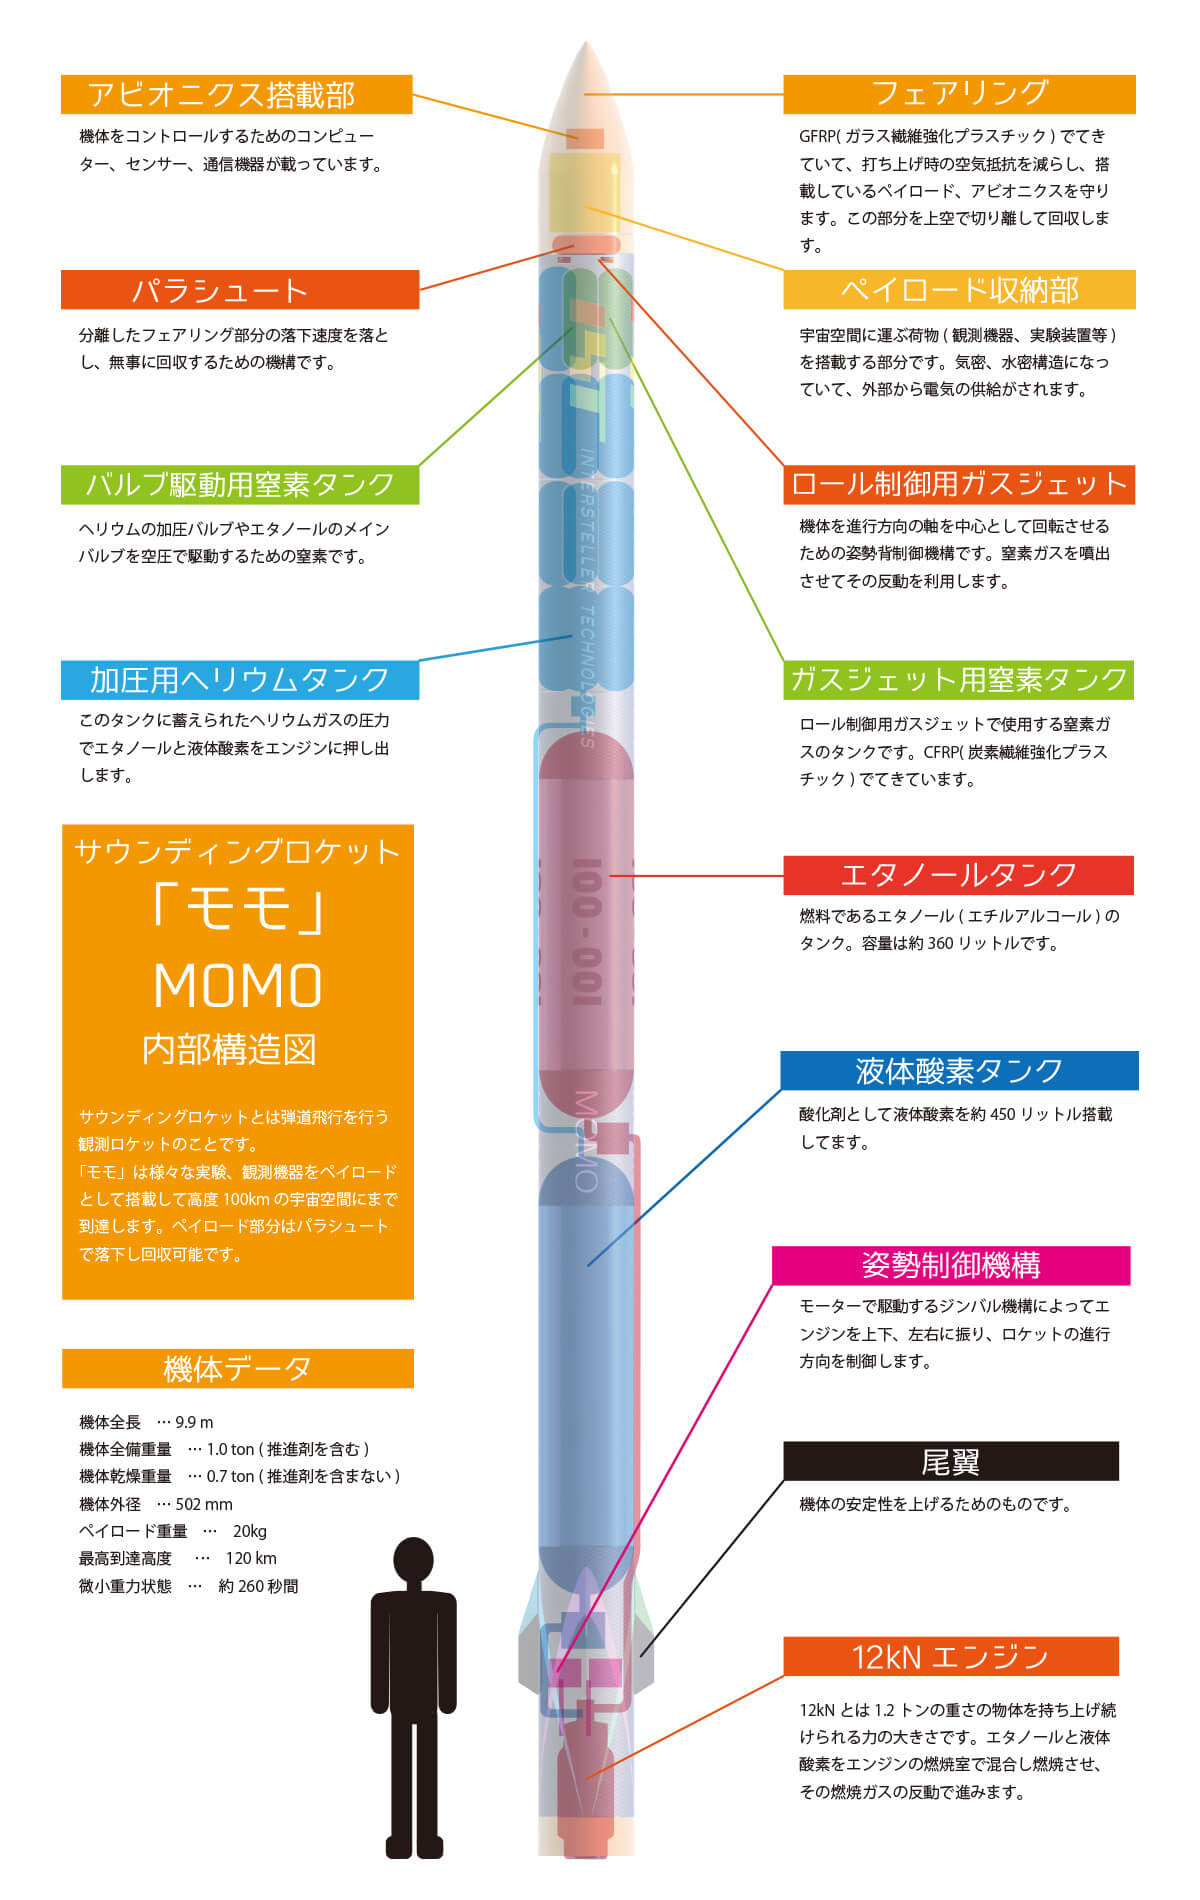
\includegraphics[width=4cm]{img/rocket-momo.jpg}
\end{figure}

7月30日に打ち上げられたのは,このMOMOの初号機である.

初号機の打ち上げはもともと,29日に行う予定であったが,濃霧のため「視程600m以上であること」という打ち上げ条件を満たせず,30日に延期した.
しかし,30日の早朝にバルブのトラブルのため打ち上げ2分前に一時中止,次のウィンドウである12:20の打ち上げを目指した.
その後も打ち上げの延期があったものの,どうにか最終ウィンドウとなる16:32に打ち上げを行った.

何度も待った上での打ち上げに,濃霧でロケットが全く見えなかったものの,見学者たちはロケットエンジンの音が遠ざかっていくのを聞き,喜んだ.


だが,その後テレメトリ消失のため,離床80秒後に地上からの指令で制御落下を行ったとの情報が入った.

30日夜に行われた会見で,打ち上げの詳細な状況が発表された.
会見の内容によると,実際には緊急停止を行ったのは離床66秒後であり,その原因はテレメトリが突然消失したからだった.
テレメトリが消失したのは高度約10kmのことで,これは最大動圧点,「max Q」に相当する.
max Qはロケット関係者の間で「機体を壊してしまうことがある大気圏内の大きなハードル」として知られており,max Qを乗り越えられるかどうか,というのは宇宙ロケットにおいて非常に重要なポイントである.
会見では,空力加熱を発生させる機体の出っ張りなどに課題があるかもしれない,と機体破損の原因について言及した一方,年内には後継機を打ち上げたい,という強気な姿勢も見られた.


この「失敗」は一部のメディアで批判的に報道された.
確かに,「宇宙空間への到達」という最終目標は達成できなかったが,それでも,何回にも及ぶ打ち上げ延期の対応や,テレメトリが取得できたところまでのデータにより得られた知見はISTにとってかけがえのないものになったのだと思う.
宇宙開発においては,サクセスクライテリアのうちフルサクセスが失敗しても,そこであきらめるのではなく,成功した部分から得られた知見を次に生かし,失敗した部分の原因究明と対策が何よりも重要だということは,宇宙開発の歴史が証明している.
インターステラの皆さんには,ぜひとも今回の「失敗」を生かし,次につなげて欲しいと思った夏休みだった.


%\section{参考文献}
%\begin{thebibliography}
%\bibitem{} \url{http://www.istellartech.com}
%\bibitem{} \url{http://fanfun.jaxa.jp/feature/detail/1104.html}
%\bibitem{} \url{http://www.itmedia.co.jp/news/articles/1003/10/news071.html}
%\bibitem{} \url{http://b-gata-diary.com/archives/2163}
%\end{thebibliography}
